\documentclass[border=10pt]{standalone}
\usepackage[scaled=0.95]{helvet}
\renewcommand{\familydefault}{\sfdefault}
\usepackage{amsmath}
\definecolor{TechCharcoal}{HTML}{202124}
\definecolor{TechNavy}{HTML}{18324B}
\begin{document}
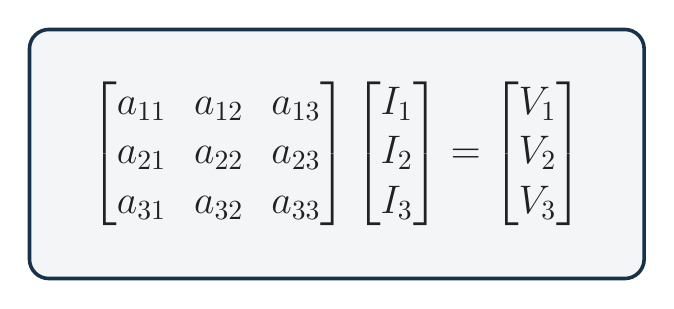
\begin{tikzpicture}
  \node[draw=TechNavy,rounded corners=7pt,line width=1.3pt,fill=TechNavy!5,
        inner xsep=22pt,inner ysep=18pt,text=TechCharcoal,font=\Large] {
    $\begin{bmatrix}
       a_{11}&a_{12}&a_{13}\\
       a_{21}&a_{22}&a_{23}\\
       a_{31}&a_{32}&a_{33}
     \end{bmatrix}
     \begin{bmatrix}I_1\\I_2\\I_3\end{bmatrix}
     =
     \begin{bmatrix}V_1\\V_2\\V_3\end{bmatrix}$
  };
\end{tikzpicture}
\end{document}
